\begin{surferIntroPage}{Површи светски рекордери}{record_chmutovoktic}{Површи светски рекордери}
    Површ се назива \emph{не-сингуларном} или \emph{глатком} ако не поседује врх 
	(такве тачке се називају \emph{сингуларитетима}). На пример, сфера или торус су 
	примери глатких површи (прве две слике).   
    Ако би се случајно бирала површ, скоро је сигурно да би била глатка. 
 \begin{center}
      \vspace{-0.2cm}
      \begin{tabular}{@{}c@{}c@{}c@{\quad}c@{}c@{}c@{}c@{}}
        \begin{tabular}{@{}c@{}}
          глатка:
        \end{tabular}
        &
        \begin{tabular}{@{}c@{}}
          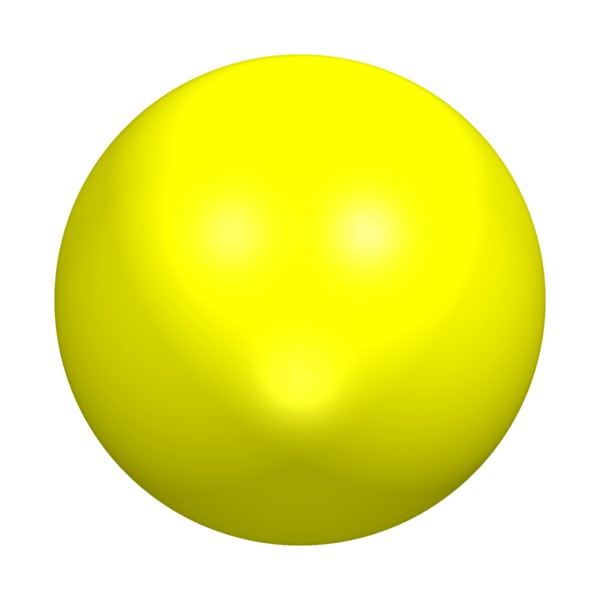
\includegraphics[width=1.1cm]{./../../common/images/kugel}
        \end{tabular}
        &
        \begin{tabular}{@{}c@{}}
          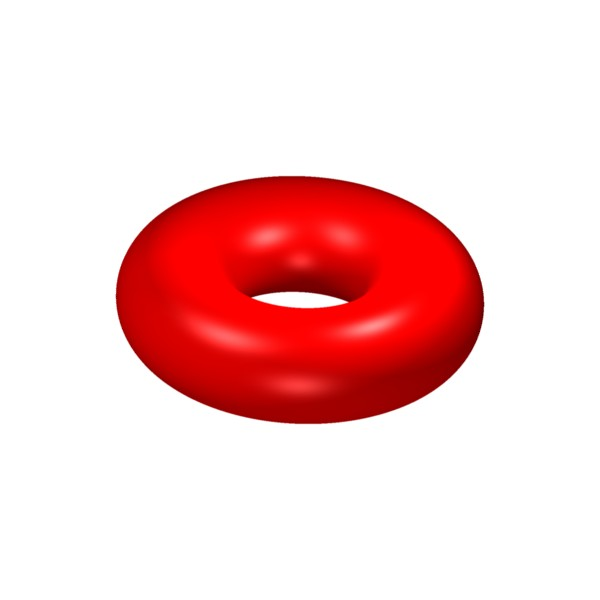
\includegraphics[width=1.1cm]{./../../common/images/torus}
        \end{tabular}
        &
        \begin{tabular}{@{}c@{}}
          више\\
          сингуларитета:
        \end{tabular}
        &
        \begin{tabular}{c@{}@{}}
          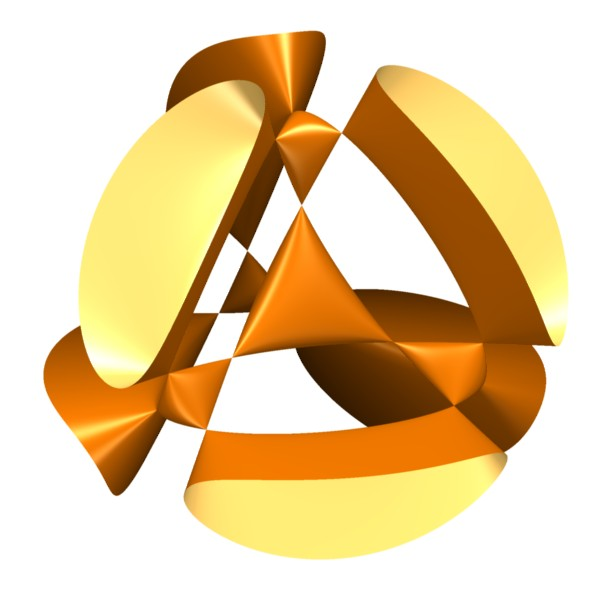
\includegraphics[width=1.1cm]{./../../common/images/kummer}
        \end{tabular}
        &
        \begin{tabular}{c@{}@{}}
          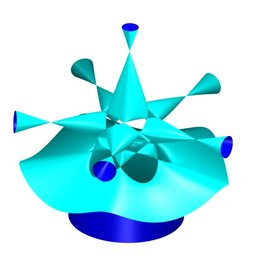
\includegraphics[width=1.1cm]{./../../common/images/togliatti}
        \end{tabular}
        &
        \begin{tabular}{c@{}@{}}
          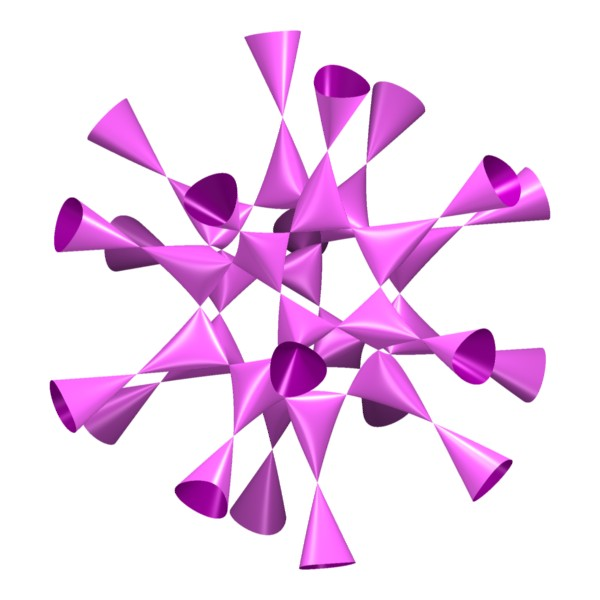
\includegraphics[width=1.1cm]{./../../common/images/barth_sextic}
        \end{tabular}
      \end{tabular}
    \end{center}
    \vspace{-0.2cm}
    Стога је површ која има сингуларитет веома специјална. Сингуларитети су најзанимљивије тачке на површи. Површи у програму SURFER су дефинисане полиномима. Највећи степен који постоји у полиному се  назива степен полинома $d$. Математичари постављају питање колико површ датог степена може 
	имати сингуларитета.
    Овај број ћемо означити са $\mu(d)$.

 Показало се да је овај број $\mu(d)$ веома тешко израчунати.
    Од $19$. века познате су вредности за $\mu(d)$  $d=1,2,3,4$, док је за  $d=5$
    овај број тек одређен осамдесетих година, за $d=6$ тек 1996.
    За вредности веће или једнаке $d\ge 7$, $\mu(d)$ је још непознат.
  
    Дакле, сваки нови светски рекорд за овај број је важан делимичан резултат. 
	Делује да је потребно много времена да би се потпуно решио овај проблем за било 
	коју вредност  $d$.\\  
	Неколико познатих резултата је дато у табели:
   \begin{center}
      \begin{tabular}{r|cccccccc|c}
        $d$ & $1$ & $2$ & $3$ & $4$ & $5$ & $6$ & $7$ & $8$ & $d$\\
        \hline
        \hline
        \rule{0pt}{1.2em}$\mu(d)\ge$ & $0$ & $1$ & $4$ & $16$ & $31$ & $65$ &
        $99$ & $168$ & 
        $\approx \frac{5}{12}d^3$\\[0.3em]
        \hline
        \rule{0pt}{1.2em}$\mu(d)\le$ & $0$ & $1$ & $4$ & $16$ & $31$ & $65$ &
        $104$ & $174$ & $\approx \frac{4}{9}d^3$
      \end{tabular}
    \end{center}
\end{surferIntroPage}
